\section{Python in High-Performance Computing}

\subsection{Sum of ranks}
The sum of ranks code performs a ring-based communication among the processes using MPI. In my implementation each process sends or receives data from or to its neighbors based on its rank. The process are divided in two disjointed groups, based on if their rank number is even or odd. This two groups are then alternating between sending and receiving. Each process has a local sum variable that sums up all the values and sends the last received rank to its neighbor with the \texttt{dest=(rank + 1) \%size
}  After the number of rounds equal to the number of processes, each process sum variable holds the sum of all ranks. Because this version of sum of ranks was implemented with \texttt{mpi4py}, there are two possible ways to implement this, one using the pickle-based communication of generic Python objects and the other the near C-speed direct array communication. These are the differences in implementation between the two:
\begin{itemize}
	\item \textbf{Pickle-based (lowercase)}: In this version you can send generic python object making the implementation straight forward. One can just put the generic python object and the function call and then save the return value of the receive function in an other variable.
	\item \textbf{Direct-array (uppercase)}: In this version the communication is done by using a buffer-like object, where the arguments need to be specified explicitly by using a tuple for example \texttt{[data, MPI.DOUBLE]} and also returns a tuple by using refernces and not a specific return statement. 
\end{itemize}

\subsection{Ghost cells}
This program is an reimplementation of the ghost cells in Project 4 in mpi4py. We construct a cartesian grid dynamically using the \texttt{MPI.Compute\_dims} function. Each process sends its ghost cells to its neighbours (north, east, south, west). The communication is done using the \texttt(Sendrecv), where the ghost cells are send in one direction and at the same time received from the opposite one.

\begin{lstlisting}[language=Python, label=lst:ghost, caption=Ghost cell Sendrecv example]
# S:left/R:right
recv_temp = np.empty(SUBDOMAIN, dtype=np.float64)
domain_send = DOMAINSIZE + 1
domain_recv = DOMAINSIZE + (SUBDOMAIN + 1)
comm_cart.Sendrecv(
    [data[domain_send:], 1, T_col],
    dest=rank_left,
    sendtag=0,
    recvbuf=[recv_temp, MPI.DOUBLE],
    source=rank_right,
    recvtag=0,
)

data[domain_recv : domain_recv + SUBDOMAIN * DOMAINSIZE : DOMAINSIZE] = recv_temp
\end{lstlisting}
In Listing \ref{lst:ghost} an example \texttt{Sendrecv} is shown, where we assign a temporary variable for the incoming buffer, set the starting point of the domain of the continously stored data for both the receiving and sending ghost cells. Subsequently the data is send and received using a costume type named \texttt{MPI\_Datype T\_col}. Finally we put the received data into the local matrix.
\begin{figure}[H]
	\centering
		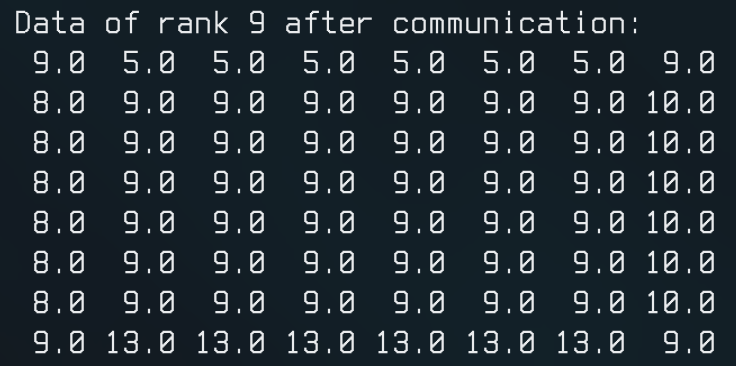
\includegraphics[width=0.8\textwidth]{./media/ghost.png}
		\caption{Output for ghost cells exchange for rank 9 with 16 processes}
		\label{fig:ghst}
\end{figure}

\subsection{A self-scheduling Parallel Mandelbrot}
The manager-worker paradigm handles the workload by dynamically efficiently distributing it among the process. This is especially useful when we deal with irregular workloads, such as the Mandelbrot set. My implementation uses a queue where all the subbatches are stored and as soon a process is done with the subbatch the next one in the queue is assigned to the worker, which in our case is just a process. This ensures efficient load is dynamically redistributed depending on availability of the worker. This comes at a cost of having higher communication overhead due to having more data exchanges and the manager can potentially act as a bottelneck. \newline 
For our scaling analysis the Mandelbrot domain is fixed and of sizes $4001\times4001$. We split the workload into 50 and 100 tasks respectivelly. In Figure \ref{fig:manager-worker} we can observe that execution time decreases significantly when the number of workers is increased. Beginning from 8 workers onwards we can see that the efficiency starts to decrease to do increased communication overhead, compared to workload per worker.
Looking at the different number of tasks, the blue line indicating a 100 tasks scales slightly better in this case the granurality results in a better load balancing which is counter acted by the prevously mentioned costs. This result shows that the load balancing and the cost pretty much offset and there is not a significant difference between the number of tasks in the case of the mandelbrot set.
\begin{figure}[H]
	\centering
		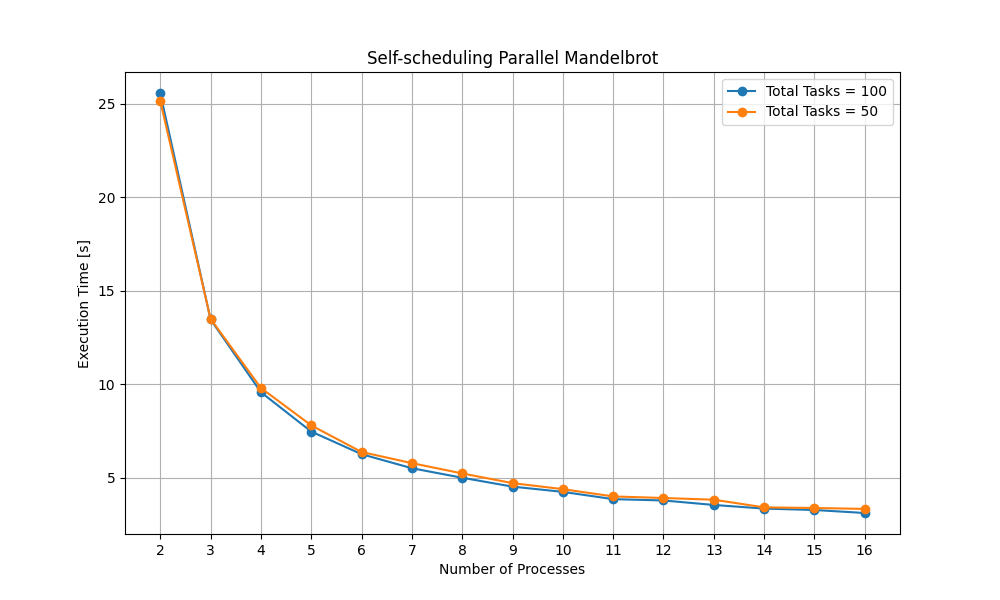
\includegraphics[width=\textwidth]{./media/manager-worker.png}
		\caption{Manager Worker scheme scaling with different number of tasks}
		\label{fig:manager-worker}
\end{figure}
